\documentclass[11pt, a4paper,spanish]{article}
\usepackage[spanish,activeacute]{babel}
\usepackage[utf8]{inputenc}
\usepackage{caratula}
\usepackage[ruled,vlined,boxed,commentsnumbered]{algorithm2e}
\usepackage{graphicx}
\usepackage{fancyhdr}
\usepackage{amsfonts}
\usepackage{amssymb}
\usepackage{amsmath}
\usepackage{hyperref}
\usepackage{float}
\usepackage{color}

% Permite colocar tablas (y figuras) una al lado de la otra. Si no se usa este 
% paquete, la única opción de LáteX es colocar las tablas y figuras una debajo de
% la otra.
\usepackage{subfigure}
% Permite combinar celdas en las tabla.
\usepackage{multirow}
% Se define la constante para el color utilizado en los comentarios del 
% pseudocódigo.
\definecolor{verde}{rgb}{0, 0.39, 0}
\usepackage{hyperref}
% Esta instrucción permite especificar un 'espaciado entre párrafos' diferente al 
% valor por defecto. El valor por defecto de LáteX para el espaciado de párrafos
% hace que éstos se encuentren demasiado arrimados unos con otros.
\setlength{\parskip}{2.5mm}
% Para tachar factores.
\usepackage{cancel}
%\usepackage[ruled,vlined,boxed,commentsnumbered]{algorithm2e}

% Encabezado y Pie de pagina
\pagestyle{fancy}
\fancyhf{}
%\fancyfoot[L]{\leftmark}
\fancyhead[L]{Ingeniería del Software 1}
\fancyhead[R]{Trabajo Pr\'actico 1}
\fancyfoot[R]{\thepage}


\begin{document}

% ------------ CARATULA ------------
     

        \materia{Ingeniería del Software 1}

        \submateria{1er cuatrimestre 2014}

    \titulo{Grupo 8: \\Trabajo Práctico 1}

%       \subtitulo{}

%       \fecha{9-04-2014}

    \integrante{Cangiani Agustín}{344/09}{cangiani@gmail.com}

    \integrante{Di Alessio Adrian}{631/06}{adrianalejandro86@hotmail.com}

    \integrante{Grosso Daniel}{694/08}{dgrosso@gmail.com}

    \integrante{Livorno Carla}{424/08}{carlalivorno@hotmail.com}
    
    \integrante{Pino Daniel}{556/07}{jdanielpino@gmail.com}

        \maketitle

        \pagebreak
 

% ------------ INDICE ------------

    \thispagestyle{empty}
    \tableofcontents
    \pagebreak

% ------------ INTRODUCCIÓN ------------

\begin{section}{Introducción}
         
%
% Primera parte.
%

\begin{subsection}{Descripción general}
Lo que sigue es una descripción general de lo que hemos interpretado a partir del enunciado del trabajo. Los detalles relativos a hipótesis y presunciones se explican en la sección siguiente.

El objetivo es la construcción de un sistema informático capaz de administrar y facilitar el uso de la nueva \emph{red de ciclovías} del distrito de \emph{Mar Chiquita}. La propuesta aspira a estimular el uso de bicletas como medio de transporte alternativo, y de esta forma se espera aliviar la red de transporte público, diminuir la circulación de autos particulares y reducir los altos niveles de sedimentarismo promoviendo la actividad física mediante el uso de la bicicleta.

La red de ciclovías está compuesta por \emph{estaciones} donde se almacenan las bicletas disponibles para los usuarios. Estas estaciones se distribuyen en diversos puntos estratégicos del distrito. Cada estación tendrá asignada un número determinado de bicicletas y por lo menos un empleado que las administra.

Se distinguen dos tipos de estaciones: \emph{periféricas} y \emph{centrales}. Las estaciones periféricas se ubican naturalmente en la periferia de la ciudad y suponemos que funcionan mayormente como puntos de salida y llegada desde las estaciones centrales por lo tanto, inferimos que también cuentan con horarios de gran demanda(presumiblemente por las mañanas). Las estaciones centrales son las de mayor demanda en los horarios centrales.

Los empleados en las estaciones atienden a los usuarios registrados que solicitan y devuelven las unidades. Estos empleados accederán al flamante sistema a través de Internet, y registrarán todos los movimientos de las estaciones que tienen a su cargo, tales como registrar nuevos usuarios, registrar los préstamos y devoluciones de unidades, recibir y atender a los camiones destinados al desplazamiento de bicicletas entre estaciones, etc. El sistema también puede emitir alertas y notificaciones para estos encargados.

El flamante sistema contará con un mecanismo de penalización para aquellos usuarios que no devuelvan las unidades en tiempo y forma según un normativa a definir por el Gobierno. Además ningún Usuario podrá tener en préstamo más de una bicicleta.

Existirá un sistema soporte o \emph{Call Center} con acceso permanente al sistema central, que permitirá a las estaciones continuar operando cuando pierdan conexión a Internet. En estos casos, los empleados de las estaciones podrán comunicarse con este centro alternativo para registrar las operaciones de sus terminales y hacer las consultas pertinentes.

Mencionamos por último que las operaciones registradas en el sistema permitirán realizar todo tipo de cómputos estadísticos con el fin de mejorar las decisiones a futuro que afecten el funcionamiento del sistema. Para ello, el sistema ofrecerá una interfaz de consulta que se describe más adelante.

\end{subsection}

\begin{subsection}{Listado de fenómenos y objetivos}
Lo que sigue es un listado con los \emph{fenómenos} más relevantes del proyecto:

\begin{itemize}
\item El usuario se registra vía Internet.
\item Si no está penalizado, el usuario registrado puede retirar solo una bicicleta en cualquiera de las estaciones.
\item Ningún usuario puede retirar más de una bicicleta.
\item El usuario debe entregar una bicicleta en uso en cualquiera de las estaciones en el plazo de una hora.
\item Los usuarios que no devuelvan las bicicletas en tiempo y forma serán penalizados.
\item Un usuario penalizado no puede retirar una bicicleta.
\item Hay dos tipos de estaciones: periféricas y centrales.
\item Las estaciones centrales tienen su mayor demanda entre las 17 y 19hs(hora pico).
\item Las estaciones centrales tienen la mayor demanda en determinadas franjas horarias.
\item Las estaciones periféricas tienen su mayor demanda presumiblemente por las mañanas.
\item Poder solicitar reposición de bicicletas.
\item Conocer la disponibilidad de bicicletas.
\item Camiones transportarán bicicletas de una estación a otra.
\item Seguridad en el resguardo de identidad.
\item Almacenamiento de datos para estadísticas.
\item Cualquier persona puede comprobar online disponibilidad de bicicletas para cualquiera de las estaciones.
\item El usuario solicita a empleado de una estación una bicicleta.
\item El usuario consulta disponibilidad de bicicletas por internet.
\item El empleado consulta disponibilidad de bicicletas.
\item El empleado valida la registración de un usuario. 
\item El empleado puede ver si un usuario esta penalizado.
\item El empleado actualiza sistema (stock de bicicletas bicicletas, estado del usuario).
\item El empleado entrega bicicleta al usuario.
\item Ante déficit de bicicletas en una o varias estaciones, el sistema determinará qué bicicletas desplazar de una estación a otra, según número de unidades en cada estación, bicicletas en uso y su destino, etc.
\item El sistema almacenará los datos de todos los movimientos para eventuales cómputos estadísticos.
\end{itemize}

Lo siguiente es la lista de \emph{objetivos blandos} considerados:

\begin{itemize}
\item \emph{``Reducir el sobrepeso en la población.''}
\item \emph{``Aliviar el transporte público y reducir el número de autos particulares.''}
\item \emph{``Sistema escalable.''}
\item \emph{``Minimizar el tiempo de espera de los usuarios en las estaciones.''}
\end{itemize}

Cada uno de estos objetivo blandos son tales por tratarse de cuestiones relativas a preferencias o aspiraciones de situaciones ideales, pero que de ninguna forma el sistema puede garantizar en todo momento.

\end{subsection} 

\begin{subsection}{Hipótesis y presunciones}
Describimos a continuación las hipótesis y presunciones 
\begin{itemize}
\item \textbf{Consultas de disponibilidad}: no se requiere de registración para consultar disponibilidad de unidades en todas las estaciones. Cualquier persona con acceso a la web podrá consultar la disponibilidad de unidades en todas las estaciones. 

\item \textbf{Registración de nuevos usuarios}: los usuarios podrán registrarse vía web, o acercándose a cualquier estación terminal a través del empleado si la estación cuenta con internet o bien comunicándose con el Callcenter desde la estación si no hay internet. Un usuario mismo no puede registrarse dos veces.

\item \textbf{Unidades sin identificación}: las bicicletas no tendrán ningún tipo de identificación. Considerando que todas las unidades son exactamente iguales, la introducción de un \emph{id} sumaría una complejidad innecesaria en el sistema sin generar ningún benefició.

\item \textbf{Desplazamiento de unidades entre estaciones}: la logística para el desplazamiento de unidades entre estaciones correrá por cuenta del sistema. Éste determinará de dónde retirar unidades y hacia dónde desplazarlas. Los camiones utilizarán esta información para el transporte de las unidades.

\item \textbf{Determinación del umbral de unidades en cada estación}: este valor determina el número de bicicletas apropiado para responder a la demanda de unidades en las distintas franjas horarias del día. Estará determinado por los cómputos estadísticos de uso y funcionamiento. En principio, se definen franjas horarias en las cuales se espera que cada estación cuente con un número determinado de unidades. Cuando el número de bicletas se encuentra por debajo de este umbral, el sistema dispará altertas automáticas a la empresa transportista solicitando más unidades. Como el concepto de umbral varía a lo largo del día, el mismo incluye la movilización de bicicletas al fin del mismo para cubrir la demanda de bicicletas al inicio del día siguiente, eventos especiales, etc.

\item \textbf{Normativa para las penalizaciones}: la normativa para las penalizaciones correrá por cuenta del gobierno de la ciudad, el cual puede consultar en el sistema a los usuarios incumplidores. Será el gobierno el que determine las penas y/o multas para estos usuarios y posteriormente si estas son resueltas, retirar las sanciones.

\item \textbf{Almacenamiento de datos y cómputos estadísticos}: el sistema ofrece una interfaz de consulta para el cálculo de estadísticas, basado en el registro de todas las operaciones en cada una de las terminales. Estos cómputos estarán a cargo del gobierno de la ciudad, pero también existe la posibilidad de configurar elementos de cálculo en el sistema mismo.

\item \textbf{Sistema de soporte basado en \textit{call-center}}: cuando por algún motivo una estación terminal pierda conexión a Internet, podrá continuar operando con el sistema comunicándose telefónica con un centro de operaciones alternativo. A través del mismo, el Encargado de la terminal puede realizar las mimas operaciones que normalmente realizaría si tuviera internet.

\item \textbf{Espera de no mayor a 40 minutos}: el sistema garantiza que se hará todo lo posible para reducir el tiempo de espera, pero de ninguna manera asegura que la espera será menor a determina cantidad de minutos.

\end{itemize}
\end{subsection}
\end{section}
\pagebreak

% ------------ ESENARIOS POSIBLES ------------

\begin{section}{Escenarios}
        
\begin{subsection}{Registración de un usuario}

El usuario se conecta a internet con algún dispositivo(pc, tablet, smartphone) y accede a la página
web del sistema de bicicletas de Mar Chiquita. Como el usuario no se encuentra registrado, necesita 
registrarse para poder acceder al servicio. Para lograrlo deberá ingresar su número de D.N.I, si dicho
número no fue registrado, el sistema le pedirá que ingrese una contraseña para proteger su cuenta. En cambio
si dicho número ya estuviese asignado el sistema le informara al usuario que deberá acercarse a cualquier
terminal del servicio para resolver su situación.

Si la registración fue exitosa, el usuario podrá ingresar de forma opcional la siguiente información:
	\begin{itemize}
	\item Nombre y apellido.
	\item Género.
	\item Dirección donde reside.
	\item Edad.
	\item Profesión.
	\item Estado civil.
	\item Correo electrónico.
	\end{itemize}

Luego el sistema le informará que su cuenta ha sido creada, faltando solamente el paso de verificación, donde
podrá acercarse a cualquier terminal con su D.N.I para confirmar la identidad del usuario. Luego de la 
verificación, el usuario estará en condiciones de retirar una bicicleta desde cualquier terminal.

Por otro lado si el sistema le hubiese informado que su D.N.I ya se encuentra registrado, el sistema le pedirá
que vaya a cualquier terminal para verificar su identificación y corregir su situación.
\end{subsection} 

\begin{subsection}{Retiro de una bicicleta}

\end{subsection} 

\begin{subsection}{Devolución de una bicicleta}

\end{subsection}

\begin{subsection}{Chequeo de stock de bicicletas en una terminal}

\end{subsection}

\begin{subsection}{Una estación se queda sin acceso a internet}

\end{subsection}

\begin{subsection}{Falla en la devolución de una bicicleta}

\end{subsection} 

\begin{subsection}{Un día en la empresa de transporte de bicicletas}

\end{subsection}

\begin{subsection}{Un día en el centro de estadísticas}

\end{subsection}
\end{section}
\pagebreak

% ------------ DIAGRAMA CONTEXTO ------------

\begin{section}{Modelo de agentes}
        

\end{section}
\pagebreak
% ------------ DIAGRAMA OBJETIVOS ------------
\begin{section}{Modelo de objetivos}
        \begin{subsection}{Diagrama de objectivos}
La figura \ref{fig:diagrama_objetivos} puede verse el diagrama de objetivos propuesto, que describe todos los objetivos del problema de las ciclovías.

\begin{figure}[H]
        \centering
        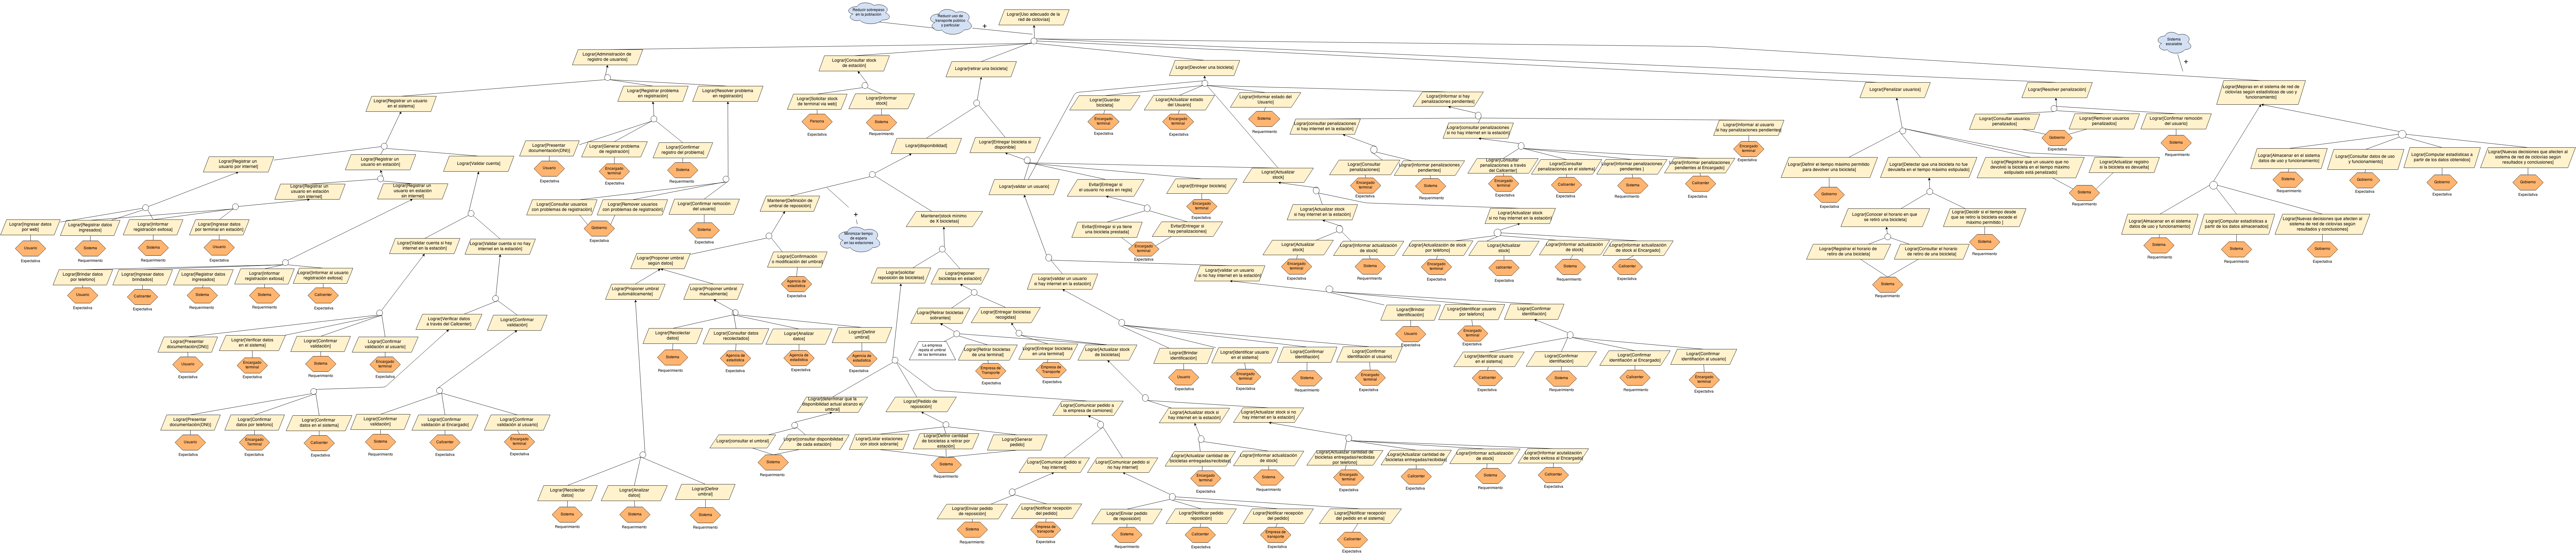
\includegraphics[angle=90,width=\textwidth,height=\textheight,keepaspectratio]{imagenes/diagrama_de_objetivos.png}
        \caption{diagrama de objetivos}
        \label{fig:diagrama_objetivos}
\end{figure}

\begin{figure}[H]
        \centering
        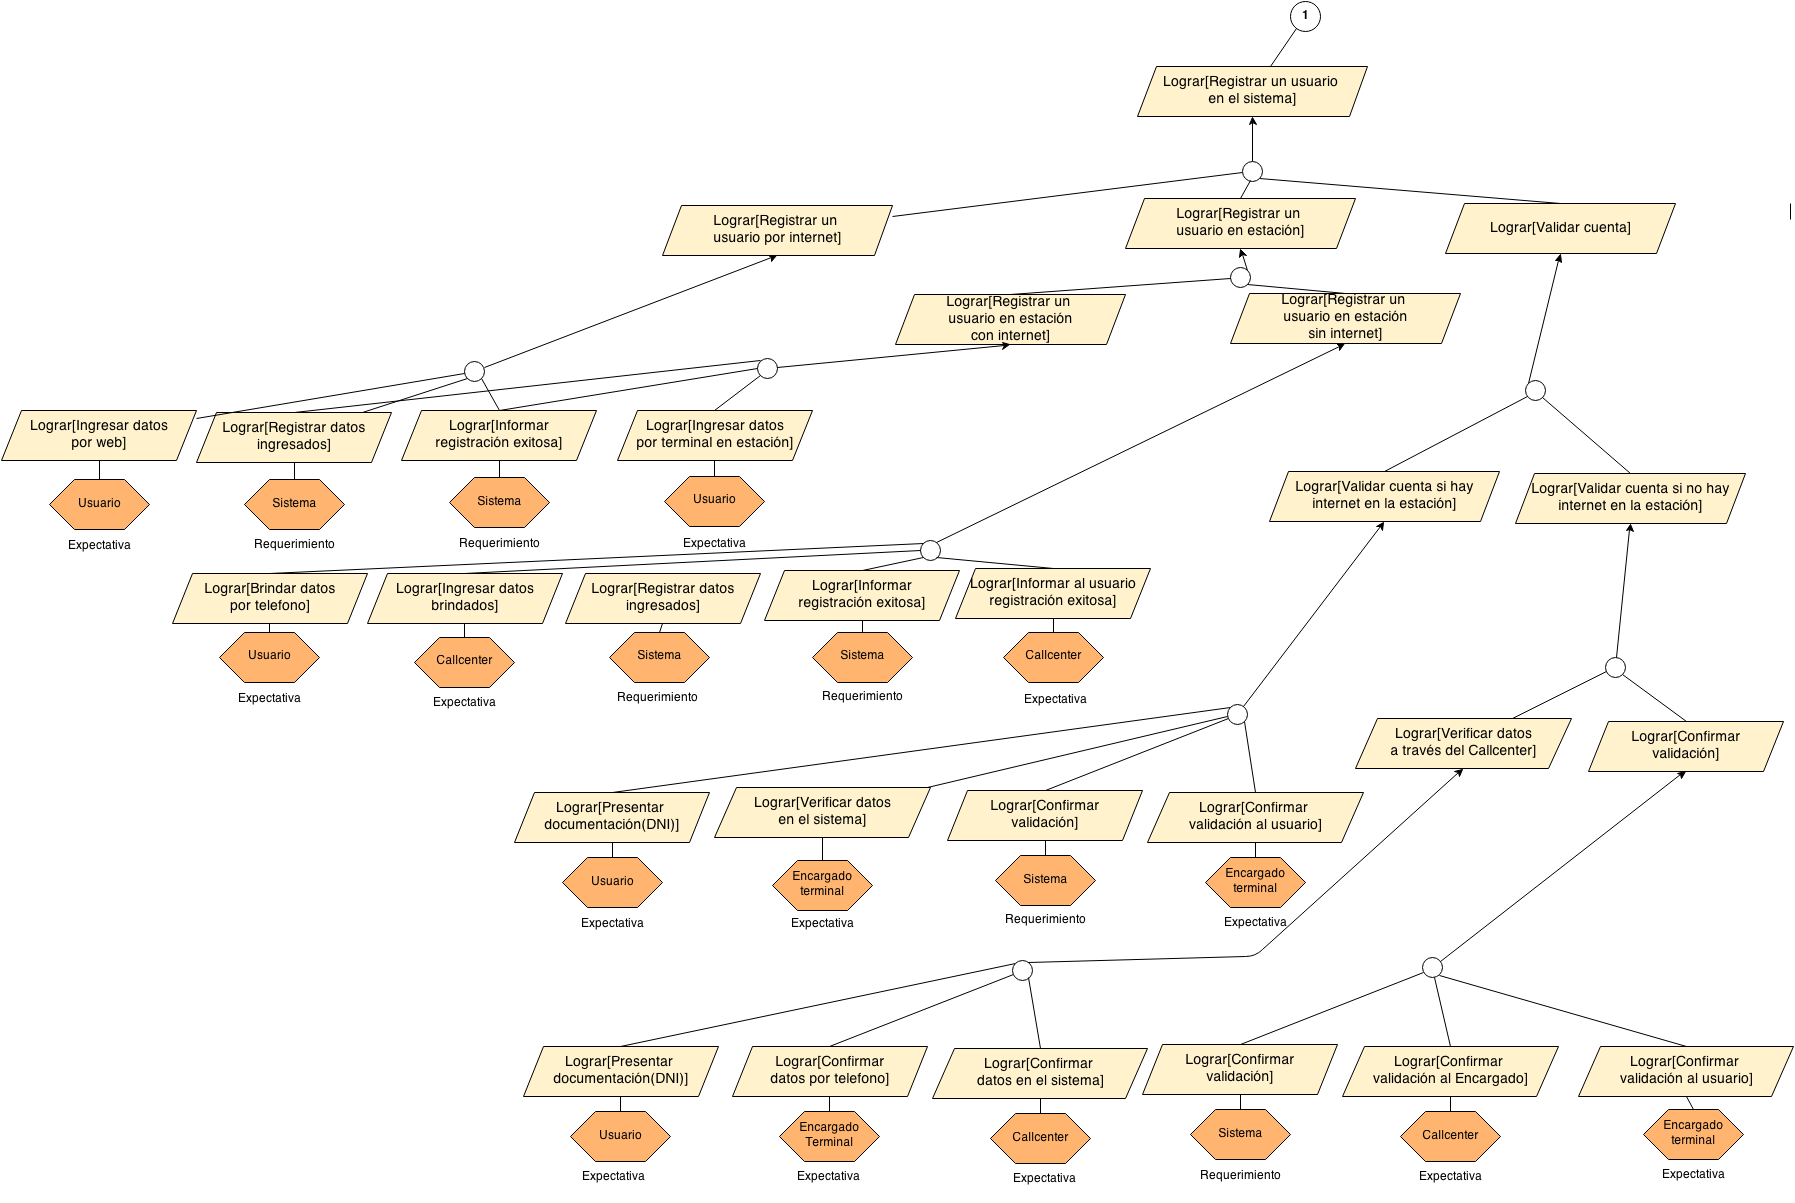
\includegraphics[angle=90,width=\textwidth,height=\textheight,keepaspectratio]{imagenes/do_1.png}
        \caption{diagrama de objetivos - 1}
        \label{fig:diagrama_objetivos_1}
\end{figure}

\begin{figure}[H]
        \centering
        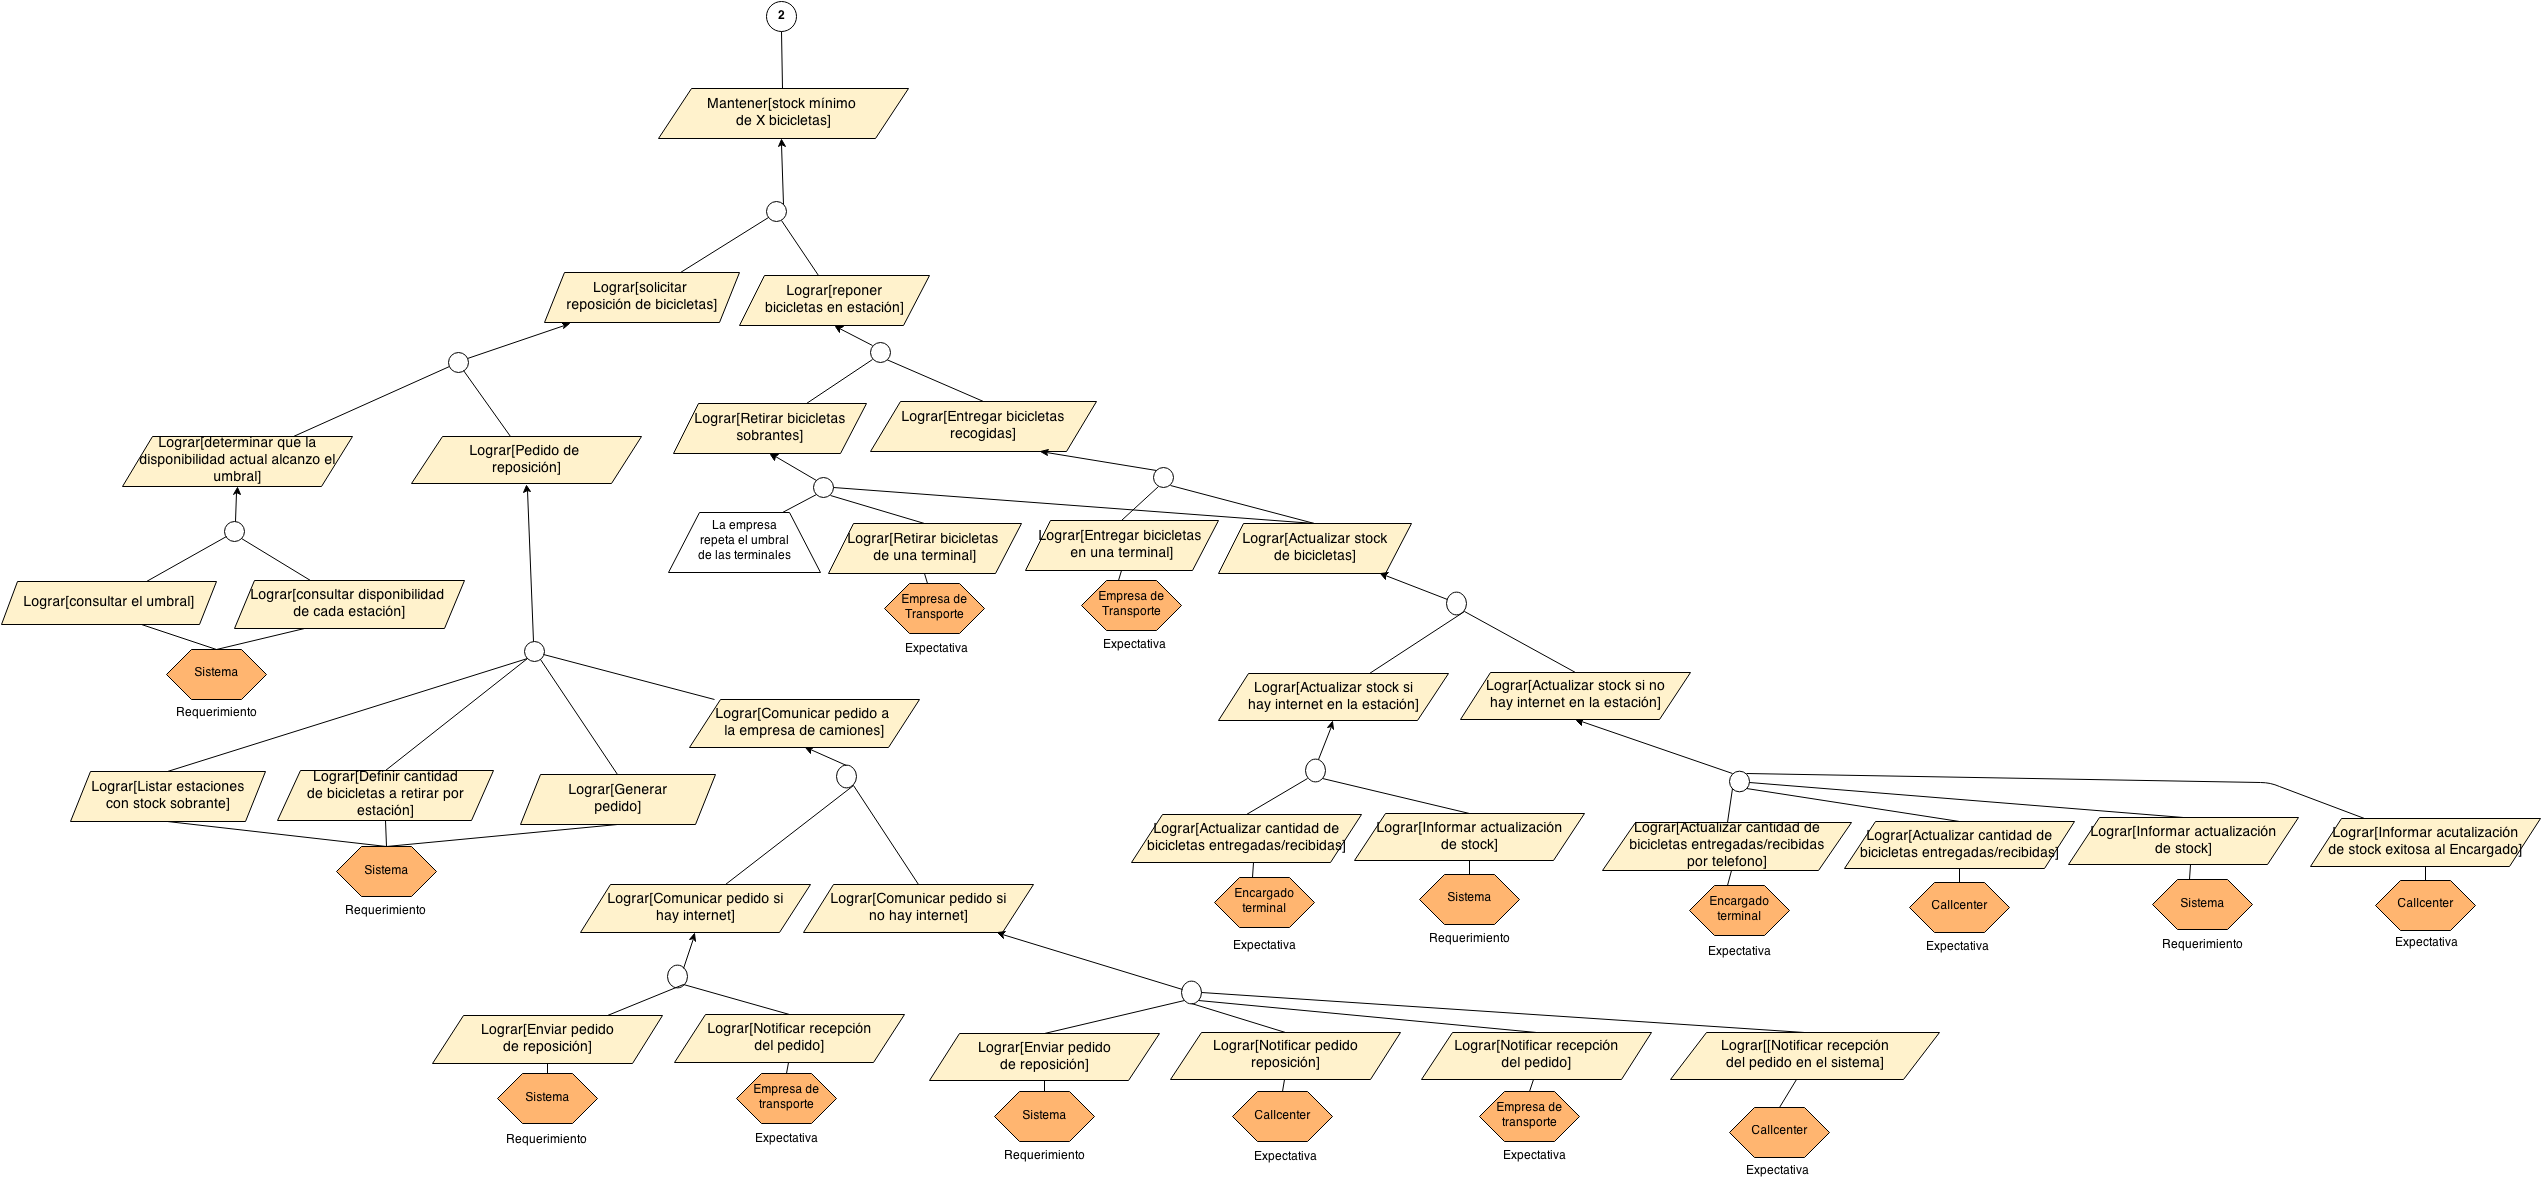
\includegraphics[angle=90,width=\textwidth,height=\textheight,keepaspectratio]{imagenes/do_2.png}
        \caption{diagrama de objetivos - 2}
        \label{fig:diagrama_objetivos_2}
\end{figure}


\begin{figure}[H]
        \centering
        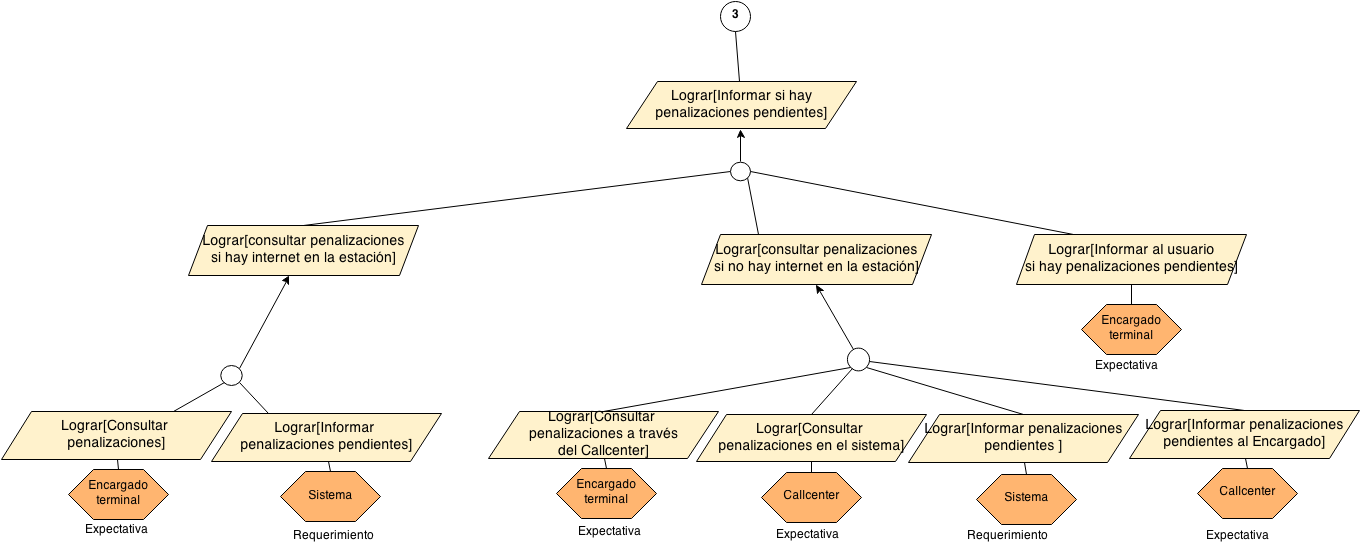
\includegraphics[angle=90,width=\textwidth,height=\textheight,keepaspectratio]{imagenes/do_3.png}
        \caption{diagrama de objetivos - 3}
        \label{fig:diagrama_objetivos_3}
\end{figure}

\begin{figure}[H]
        \centering
        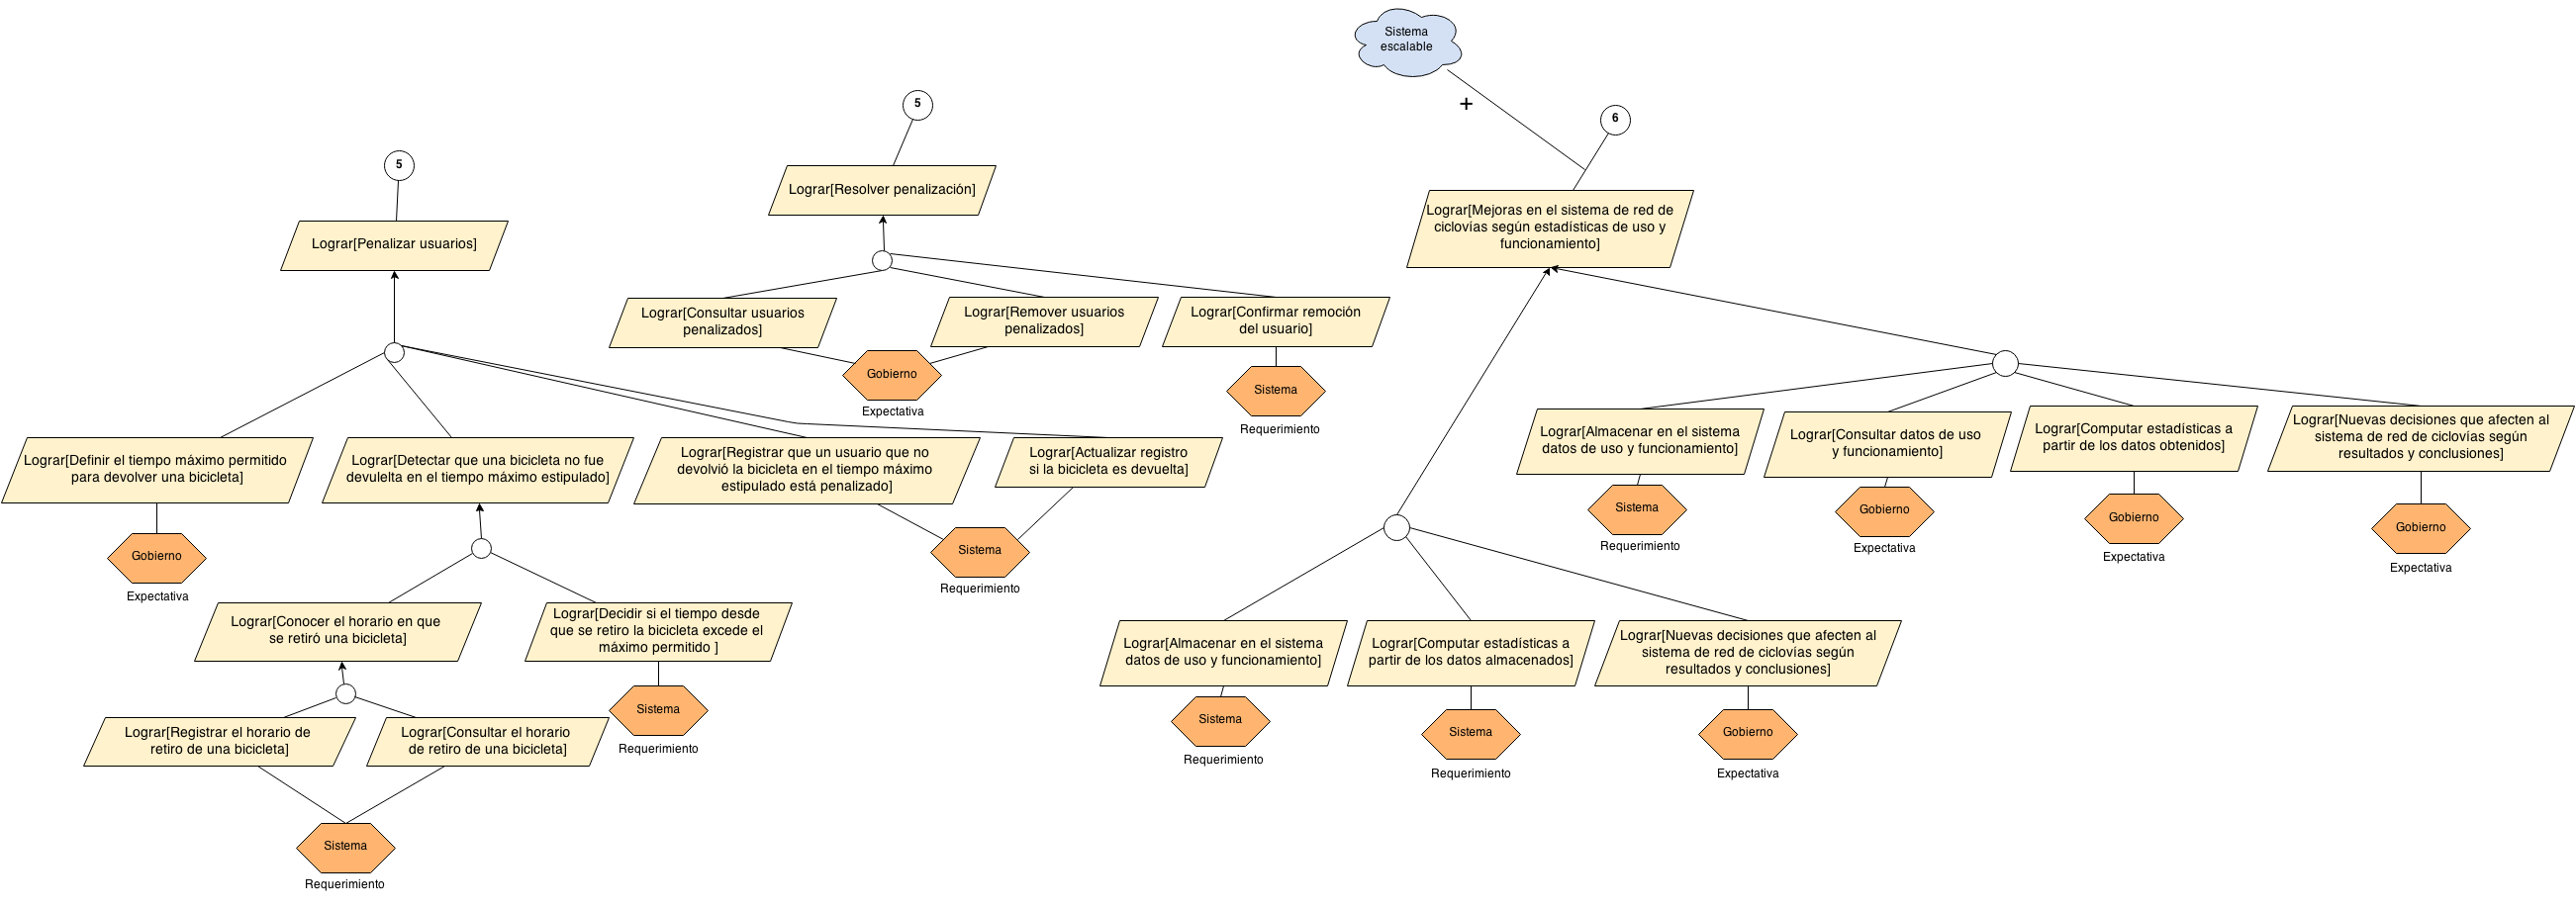
\includegraphics[angle=90,width=\textwidth,height=\textheight,keepaspectratio]{imagenes/do_4-5-6.png}
        \caption{diagrama de objetivos - 4 5 6}
        \label{fig:diagrama_objetivos_4_5_6}
\end{figure}
%\begin{figure}[H]
%	
%	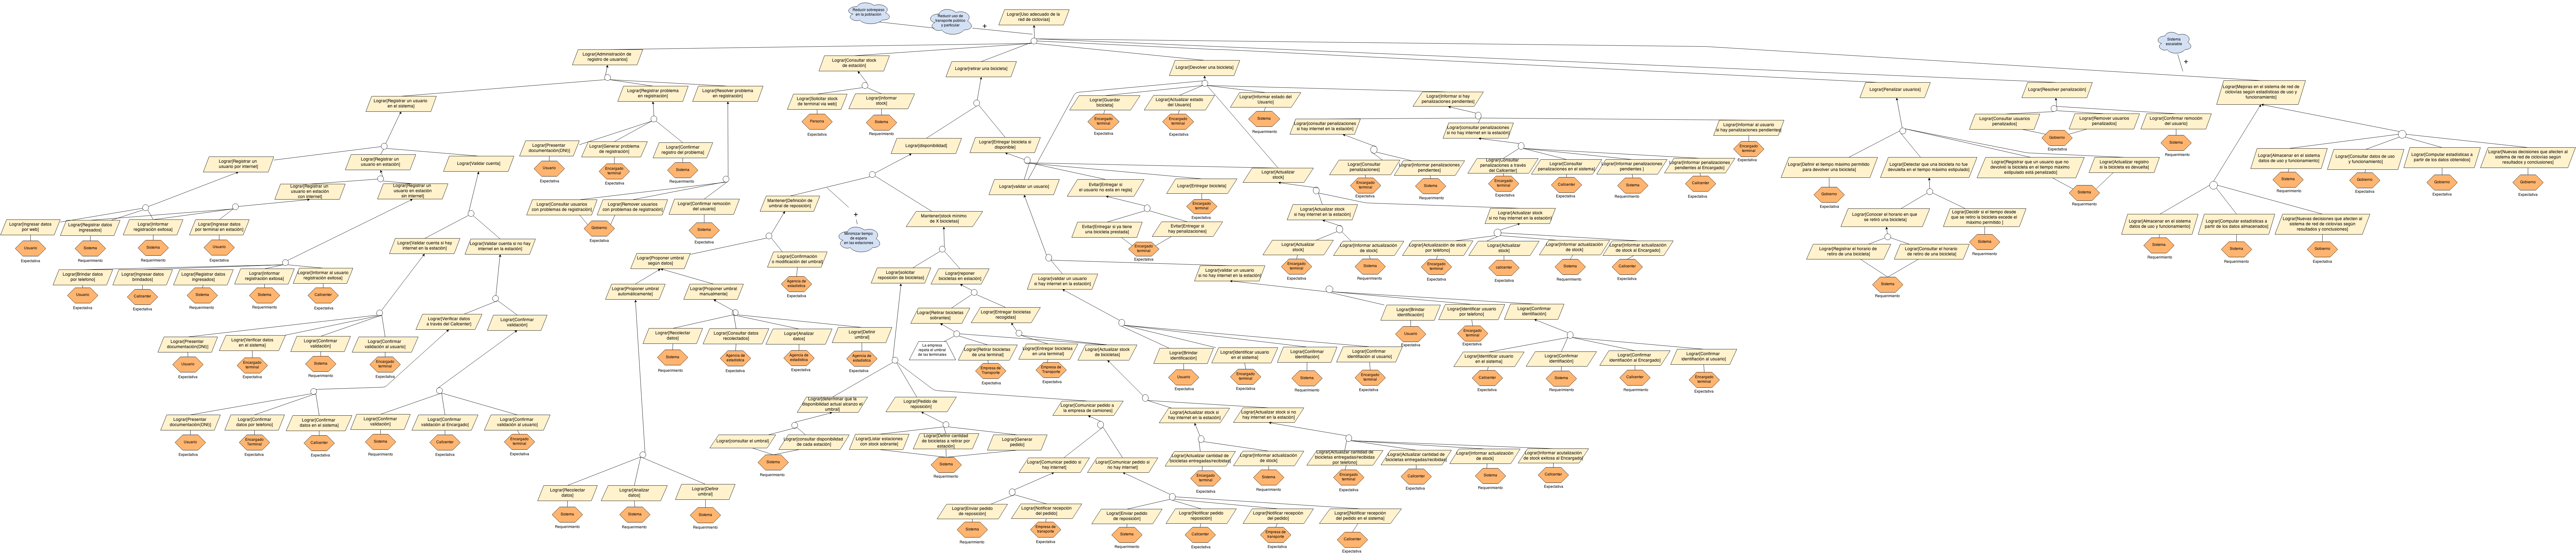
\includegraphics[scale=0.47]{imagenes/diagrama_de_objetivos.png}
%	\caption{diagrama de contexto}
%	\label{fig:diagrama_objetivos}
%
%\end{figure}

\end{subsection}

%\begin{subsection}{Análisis de objetivos}

%\end{subsection}
\end{section}\begin{flushleft}\end{flushleft}

% ------------ REFERENCIAS ------------
    \pagebreak
%    \section{Referencias}
%        



\end{document}